% Created 2021-04-21 Wed 21:00
% Intended LaTeX compiler: xelatex
\documentclass[12pt]{article}
\usepackage{graphicx}
\usepackage{grffile}
\usepackage{longtable}
\usepackage{wrapfig}
\usepackage{rotating}
\usepackage[normalem]{ulem}
\usepackage{amsmath}
\usepackage{textcomp}
\usepackage{amssymb}
\usepackage{capt-of}
\usepackage{hyperref}
\usepackage{minted}
\usepackage{amsmath}
\usepackage{amssymb}
\usepackage{setspace}
\usepackage{subcaption}
\usepackage{mathtools}
\usepackage{xfrac}
\usepackage[margin=1in]{geometry}
\usepackage{marginnote}
\usepackage[utf8]{inputenc}
\usepackage{color}
\usepackage{epsf}
\usepackage{tikz}
\usepackage{graphicx}
\usepackage{pslatex}
\usepackage{hyperref}

\usepackage{beton}
\usepackage{euler}
\usepackage[OT1]{fontenc}

\usepackage{textgreek}
\renewcommand*{\textgreekfontmap}{%
{phv/*/*}{LGR/neohellenic/*/*}%
{*/b/n}{LGR/artemisia/b/n}%
{*/bx/n}{LGR/artemisia/bx/n}%
{*/*/n}{LGR/artemisia/m/n}%
{*/b/it}{LGR/artemisia/b/it}%
{*/bx/it}{LGR/artemisia/bx/it}%
{*/*/it}{LGR/artemisia/m/it}%
{*/b/sl}{LGR/artemisia/b/sl}%
{*/bx/sl}{LGR/artemisia/bx/sl}%
{*/*/sl}{LGR/artemisia/m/sl}%
{*/*/sc}{LGR/artemisia/m/sc}%
{*/*/sco}{LGR/artemisia/m/sco}%
}
\makeatletter
\newcommand*{\rom}[1]{\expandafter\@slowromancap\romannumeral #1@}
\makeatother
\DeclarePairedDelimiterX{\infdivx}[2]{(}{)}{%
#1\;\delimsize\|\;#2%
}
\newcommand{\infdiv}{D\infdivx}
\DeclarePairedDelimiter{\norm}{\left\lVert}{\right\rVert}
\DeclarePairedDelimiter{\ceil}{\left\lceil}{\right\rceil}
\DeclarePairedDelimiter{\floor}{\left\lfloor}{\right\rfloor}
\def\Z{\mathbb Z}
\def\R{\mathbb R}
\def\C{\mathbb C}
\def\N{\mathbb N}
\def\Q{\mathbb Q}
\def\noi{\noindent}
\onehalfspace
\usemintedstyle{bw}
\author{Sandy Urazayev\thanks{University of Kansas (ctu@ku.edu)}}
\date{67; 12021 H.E.}
\title{Homework 3 Oracle\\\medskip
\large MATH 220 Spring 2021}
\hypersetup{
 pdfauthor={Sandy Urazayev},
 pdftitle={Homework 3 Oracle},
 pdfkeywords={},
 pdfsubject={},
 pdfcreator={Emacs 28.0.50 (Org mode 9.4.5)}, 
 pdflang={English}}
\begin{document}

\maketitle
\href{./index.pdf}{[View the PDF version]​}

\section*{Section 2.3}
\label{sec:org30d5c92}
\subsection*{Problem 1 [FOR GRADE]}
\label{sec:org8ccfe48}
We model the tank problem the following way of
\begin{equation*}
  \frac{dx}{dt}=R_{in}-R_{out}
\end{equation*}
Then
\begin{equation*}
  \frac{dx}{dt}=-\frac{2x}{200}=-\frac{x}{100}
\end{equation*}
We know the original concentration of \(1g/L\), then apply the separable
equations method
\begin{equation*}
  \int \frac{100}{x} dx = \int -1 dt
\end{equation*}
Solving it yields
\begin{equation*}
x = 200 e^{-\frac{t}{100}}
\end{equation*}
We need to find the time that will elapse before the concentration of dye in
the tank reaches \(1\%\). So
\begin{equation*}
  \frac{x(t)}{x(0)} = 0.01 \implies 0.01 = e^{-\frac{t}{100}}
\end{equation*}
Solving for \(t\) returns that \(t = 100 \ln 100\) min \(\approx 460.5\) min. 
\subsection*{Problem 4}
\label{sec:orgd535dc6}
\subsubsection*{Part (a)}
\label{sec:org5c5fa9a}
So our kinetic and potential energies are equal. Then
\begin{equation*}
  mgh = \frac{1}{2}mv^2 \implies v = \sqrt{2gh}
\end{equation*}
\subsubsection*{Part (b)}
\label{sec:org29b5076}
Recall 
\begin{equation*}
  \frac{dv}{dt} = A(h) \frac{dh}{dt} \quad\text{and}\quad \frac{dv}{dt} = av
\end{equation*}
So then because constant \(\alpha\) is contracting, the change is negative
\begin{equation*}
  A(h)\frac{dh}{dt} = -\alpha a \sqrt{2gh}
\end{equation*}
\subsubsection*{Part (c)}
\label{sec:org444f789}
Recall \(A(r) = \pi r^2\). Let \(h=3\) and \(\alpha = 0.6\). Then solving for
radius of 1m and the circular outlet radius of 0.1m, we get an equation
\begin{equation*}
  A(1)\frac{dh}{dt} = -(0.6) \times A(0.1) \sqrt{2gh}\\
  \implies \pi\frac{dh}{dt} = -0.006 \pi \sqrt{2gh}\\
  \implies \frac{dh}{dt} = -0.006 \sqrt{2gh}\\
\end{equation*}
Solving for \(t\) yields \(\approx 130.41\). 
\subsection*{Problem 9 [FOR GRADE]}
\label{sec:orgf1dee81}
\subsubsection*{Part (a)}
\label{sec:org77b8378}
See that
\begin{equation*}
  \frac{Q(5730)}{Q_0} = 0.5\\
  \implies \frac{Q_0 e^{-r(5730)}}{Q_0} = 0.5\\
  \implies e^{-r(5730)} = 0.5\\
\end{equation*}
Solve for \(r\) to get \(r = 0.00012097 yr^{-1}\) 
\subsubsection*{Part (b)}
\label{sec:org152372c}
Trivially, it would be \(Q_0 \exp{(-0.00012097t)}\), where \(t\) is measured in
years. 
\subsubsection*{Part (c)}
\label{sec:orgc28cd72}
Solve \(e^{-rt} = 0.2\) to get \(13,305yr\). 
\section*{Section 2.5}
\label{sec:org1b87d5b}
\subsection*{Problem 3}
\label{sec:orgf146454}
\begin{center}
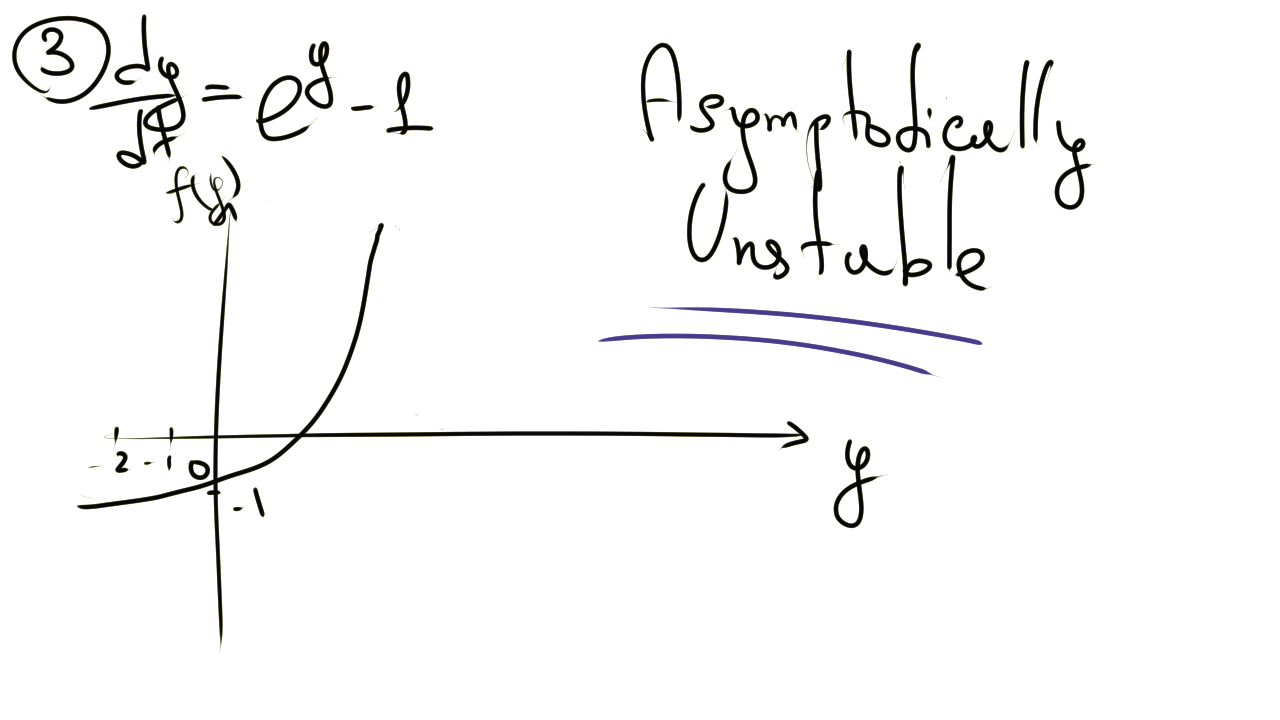
\includegraphics[width=.9\linewidth]{./d3.png}
\end{center}
\subsection*{Problem 5}
\label{sec:org5f8cb39}
\begin{center}
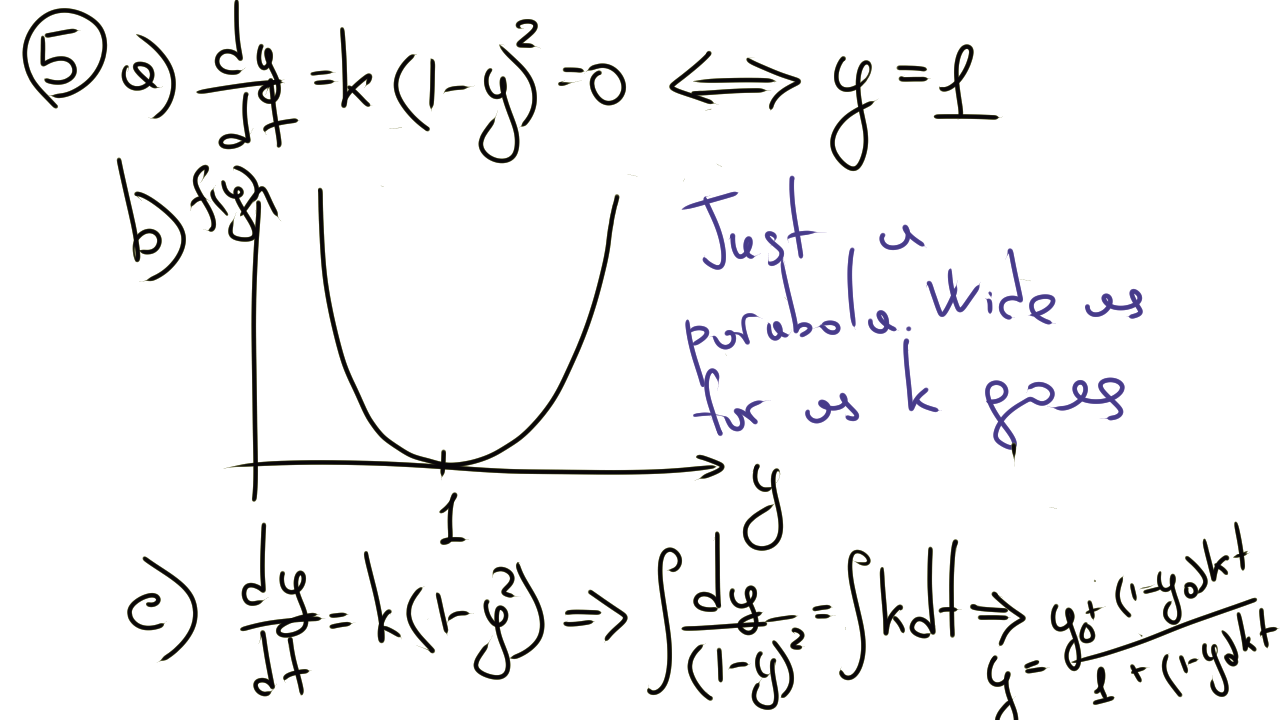
\includegraphics[width=.9\linewidth]{./d5.png}
\end{center}
\subsection*{Problem 9 [FOR GRADE]}
\label{sec:org0d49c64}
\begin{center}
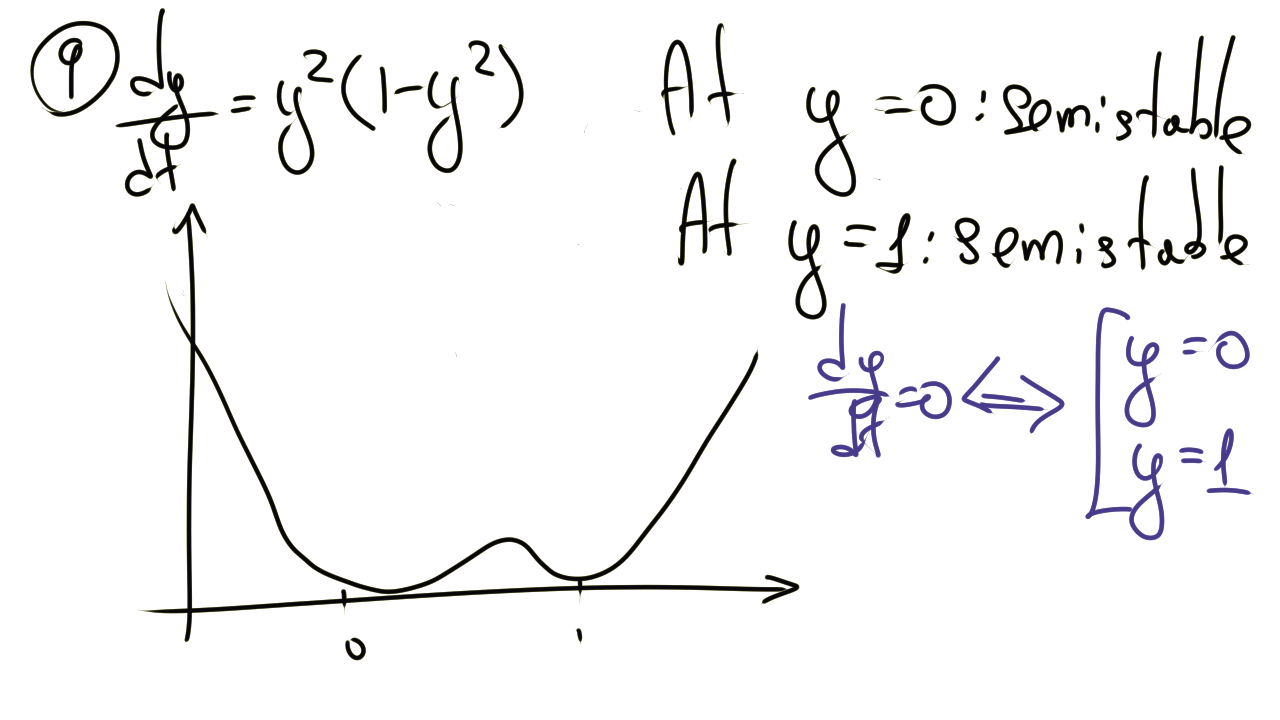
\includegraphics[width=.9\linewidth]{./d9.png}
\end{center}
\subsection*{Problem 13}
\label{sec:org8fd962a}
\begin{equation*}
  y_{1,2} = \frac{K + T \pm \sqrt{K^2 - KT + T^3}}{3}
\end{equation*}
\end{document}